\documentclass[review ]{elsarticle}
\documentclass[conference, 11pt]{IEEEtran} 
\usepackage{verbatim}
\usepackage{multirow} \usepackage{enumerate}
\usepackage{amsmath,enumerate} \usepackage{amsthm}
\usepackage{algcompatible}
\usepackage{algpseudocode}
\usepackage{algorithm}
%\usepackage{algorithmic}
\usepackage{pstricks}
\usepackage{amssymb, latexsym}
\usepackage{xfrac}
\usepackage{mathtools}
\usepackage{graphicx}
\usepackage{subfig}
\DeclareGraphicsRule{*}{mps}{*}{}
\usepackage{listings}

%specific to this document only
\usepackage{pgfplots}
\usepackage{pgfplotstable}
\pgfplotstableread{plts/experiment8b1_av.tab}\averageone
\pgfplotstableread{plts/experiment8b2_av.tab}\averagetwo
\pgfplotstableread{plts/experiment8b3_av.tab}\averagethree
\pgfplotstableread{plts/experiment8b4_av.tab}\averagefour
\pgfplotstableread{plts/experiment9a_av.tab}\stepping
\pgfplotstableread{plts/experiment9a1_av.tab}\steppingone
\pgfplotstableread{plts/experiment9a2_av.tab}\steppingtwo
\pgfplotstableread{plts/experiment9a3_av.tab}\steppingthree
\pgfplotstableread{plts/experiment9a4_av.tab}\steppingfour
\pgfplotstableread{plts/experiment9b1_av.tab}\runningone
\pgfplotstableread{plts/experiment9b2_av.tab}\runningtwo
\pgfplotstableread{plts/experiment9b3_av.tab}\runningthree
\pgfplotstableread{plts/experiment9b4_av.tab}\runningfour
\pgfplotstableread{plts/experiment9b_av.tab}\running
\pgfplotstableread{plts/experiment9c_av.tab}\costcomp
\pgfplotstableread{plts/experiment9c1_av.tab}\costcompone
\pgfplotstableread{plts/experiment9c2_av.tab}\costcomptwo
\pgfplotstableread{plts/experiment9c3_av.tab}\costcompthree
\pgfplotstableread{plts/experiment8b1_rn.tab}\runsone
\pgfplotstableread{plts/experiment8b2_rn.tab}\runstwo
\pgfplotstableread{plts/experiment8b3_rn.tab}\runsthree
\pgfplotstableread{plts/experiment8b4_rn.tab}\runsfour
\pgfplotstableset{
  create on use/density/.style={
    create col/expr={\thisrow{nodes}+\thisrow{links}}}
    }
\pgfplotstableset{
  create on use/delta/.style={
    create col/expr={\thisrow{links}*2}}
    }
\pgfplotstableset{
  create on use/nodebylinks/.style={
    create col/expr={(\thisrow{nodes}*\thisrow{links})}}
    }
\pgfplotscreateplotcyclelist{three}{% 
  every mark/.append style={fill=teal}\\% 
  every mark/.append style={fill=green}\\% 
  every mark/.append style={fill=orange}\\% 
}
\pgfplotscreateplotcyclelist{four}{%
  every mark/.append style={fill=teal}\\%
  every mark/.append style={fill=green}\\%
  every mark/.append style={fill=orange}\\%
  every mark/.append style={fill=pink}\\%
}

%%%%%%%%%%%%%

\usepackage{pgf}
\usepackage{tikz}
\usetikzlibrary{decorations.pathmorphing} % LATEX and plain TEX when using Tik Z
\usetikzlibrary{positioning}
\usetikzlibrary{er}
\usetikzlibrary{automata}
\usetikzlibrary{shapes.geometric}
\tikzstyle{vx}=[draw,circle,fill=white,minimum size=2pt, inner sep=1pt, node distance=15mm]
\tikzstyle{ex}=[draw,rectangle,fill=white,minimum size=2pt, inner sep=3pt, node distance=15mm]
\tikzstyle{bup}=[semithick, decoration={bent, aspect=.3, amplitude=4}, decorate, ->, >=stealth]
\tikzstyle{bdn}=[semithick, decoration={bent, aspect=.3, amplitude=-4}, decorate, ->, >=stealth]
\tikzstyle{BUP}=[thick, decoration={bent, aspect=.3, amplitude=8}, decorate, ->, >=stealth]
\tikzstyle{BDN}=[thick, decoration={bent, aspect=.3, amplitude=-8}, decorate, ->, >=stealth]
\tikzstyle{MUP}=[thick, decoration={bent, aspect=.3, amplitude=16}, decorate, ->, >=stealth]
\tikzstyle{MDN}=[thick, decoration={bent, aspect=.3, amplitude=-16}, decorate, ->, >=stealth]
\tikzstyle{str}=[semithick, decorate, ->, >=stealth]
\tikzstyle{cr}=[draw, circle, fill=black!25,minimum size=150pt]

%styles for plots?
\tikzstyle{bls}=[blue, solid, mark=square*]
\tikzstyle{grt}=[red, solid, mark=*]
% \paperheight=11in \paperwidth=8.5in \textheight=9.0in
% \textwidth=6.5in \voffset=-.875in \hoffset=-.875in
\newenvironment{code} {\begin {quote}\begin{footnotesize}}
    {\end{footnotesize}\end{quote}}

% \oddsidemargin 0.0 in \evensidemargin 0.0 in
\newenvironment{enumeratealpha}
{\begin{enumerate}[(a{\textup{)}}]}{\end{enumerate}}

\theoremstyle{plain}
\newtheorem{lem-rule}{Rule}
\newtheorem{thm}{Theorem}
\newtheorem{lem}{Lemma}[thm]
\newtheorem{prop}{Proposition}[thm]
\newtheorem{lprp}{Proposition}[lem]
\theoremstyle{definition}
\newtheorem{defn}{Definition}[thm]
\newtheorem{dfn}{Definitions}[thm]
\newtheorem{ldef}{Definition}
\theoremstyle{remark}
\newtheorem{smy}{Summary}
\newtheorem{note}{Note}[thm]

%algorithms commands
\algblockdefx[Case]{Case}{EndCase} %
[1] [{\em var}] {{\bfseries case} {\em #1\ } } %
{{\bfseries end case}}%
\algcblockdefx[Case]{Case}{When}{EndCase}
[1] [{\em true}] {{\bfseries when} {\em #1\ }}
{{\bfseries end case}} %

\algblockdefx[TimesDo] {DoTimes}{EndTimes}
[1] [0] {#1 times {\bfseries do}}
{{\bfseries end do}}

%subalgorithms environment
\makeatletter
\newcounter{parentalgorithm}
\newenvironment{subalgorithms}{%
%  \refstepcounter{algorithm}%
  \floatname{algorithm}{Procedure}
  \protected@edef\theparentalgorithm{\thealgorithm}%
  \setcounter{parentalgorithm}{\value{algorithm}}%
  \setcounter{algorithm}{0}%
  \def\thealgorithm{\theparentalgorithm-\alph{algorithm}}%
  \ignorespaces
}{%
  \setcounter{algorithm}{\value{parentalgorithm}}%
  \ignorespacesafterend
}
\makeatother

%code environments
\usepackage{float}
 
\floatstyle{ruled}
\newfloat{codeblock}{thp}{lop}
\floatname{codeblock}{Example}

\lstnewenvironment{rubyblock} 
{\lstset{language=Ruby, basicstyle=\small, xleftmargin=10pt, numbers=left, numberstyle=\tiny, stepnumber=2, numbersep=5pt}}
{}
% text macros
\def\cI{{\mathcal I}} \def\cR{{\mathcal R}} \def\cE{{\mathcal E}}
\def\cC{{\mathcal C}} \def\cF{{\mathcal F}} \def\cU{{\mathcal U}}
\def\cH{{\mathcal H}} \def\cD{{\mathcal D}} \def\cB{{\mathcal B}}
\def\cQ{{\mathcal Q}} \def\cV{{\mathcal V}} \def\cS{{\mathcal S}}
\def\cG{{\mathcal G}} \def\cA{{\mathcal A}} \def\cO{{\mathcal O}}
\def\cW{{\mathcal W}} \def\cL{{\mathcal L}} 

\def\bI{{\mathbb I}} \def\bO{{\mathbb O}}
\def\bC{{\mathbb C}} \def\bM{{\mathbb M}}
\def\bId{{$\mathbb I$}} \def\bOd{{$\mathbb O$}}
\def\bCd{{$\mathbb C$}} \def\bMd{{$\mathbb M$}}

\def\cId{{$\mathcal I$}} \def\cRd{{$\mathcal R$}} \def\cEd{{$\mathcal E$}} 
\def\cCd{{$\mathcal C$}} \def\cFd{{$\mathcal F$}} \def\cUd{{$\mathcal U$}} 
\def\cHd{{$\mathcal H$}} \def\cDd{{$\mathcal D$}} \def\cBd{{$\mathcal B$}} 
\def\cQd{{$\mathcal Q$}} \def\cVd{{$\mathcal V$}} \def\cSd{{$\mathcal S$}} 
\def\cGd{{$\mathcal G$}} \def\cAd{{$\mathcal A$}} \def\cOd{{$\mathcal O$}}
\def\cWd{{$\mathcal W$}} \def\cLd{{$\mathcal L$}}

\bibliographystyle {IEEEtranS}

\bibliographystyle {elsarticle-num}
\begin{document}
\title{A Simple Distributed Algorithm for Minimum Weighted Vertex Cover}
\author[gsu]{J. Paul Daigle}
\ead{j.paul.daigle@gmail.com}
\author[gsu]{Sushil K. Prasad}
\ead{sushil.prasad@gmail.com}
\address[gsu]{Department of Computer Science, Georgia State University, P.O. Box 3994, Atlanta, GA  30302-3994}
\begin{abstract} Vertex cover, a minimal set of nodes to cover all edges in a graph, is an abstraction of coverage problems in sensor networks, transportation networks, etc., and is a well-known NP-hard problem.  Minimum weighted vertex cover (MWVC) problem asks for further minimizing the cumulative weight of a vertex cover.  We present a new distributed 1-hop algorithm for the MWVC problem with theoretical and practical value.  Our first 1-hop approximation algorithm, based on matching a maximal set of non-adjacent edges, is provably 2-optimal with a communication complexity of $O(\log\Delta)$.   It compares very well with the current state-of-art in quality while significantly reducing communication cost.
\end{abstract}

\begin{keyword}Distributed Algorithms \sep Graph Algorithms \sep Vertex Cover \end{keyword}
\maketitle

\section{Introduction}

The Minimum Vertex Cover problem and its weighted variant are NP-Complete problems with several known linear time sequential algorithms that provide constant factor approximations. The existence of such algorithms suggests that it should be theoretically possible to discover a distributed or parallel algorithm to provide a constant factor approximation in constant time, however, it has been proven that no such algorithm exists\cite{1011811}. 

Here we present a distributed algorithm that provides a two-approximate solution to Minimum Weighted Vertex Cover in $O(\log\Delta)$ rounds with high probability, where $\Delta$ is the largest degree of the graph. This algorithm, based on Maximal Matchings, is the first distributed algorithm that we are aware of with a performance based on $\Delta$ rather than on the size of the graph. 

\subsection{Problem Definition}
\subsubsection{Minimum Vertex Cover (MVC)}
\label{sub:mvc}
Given an undirected Graph $G(V,E)$, a {\em Vertex Cover} of $G$ is a set of vertices $V'$ such that for each edge $e_{u,v} \in E$, $u \in V'$ or $v \in V'$. The Minimum Vertex Cover Problem is to find the smallest possible vertex cover of $G$.

\subsubsection{Minimum Weighted Vertex Cover (MWVC)}
\label{sub:mwvc}
Given an undirected Graph $G(V,E)$, where each $v \in V$ has a positive weight $w(v)$, minimize $\sum_{v \in V'} w(v)$.

%\subsubsection{Minimum (Weighted) Vertex Cover of a Hypergraph}

%Given a Hypergraph $G(V,E)$, with vertices $v \in V$ and hyperedges $e_{v_1...v_n}$, a vertex cover of $G$ is a set $V'\: | \: \forall e \in E,\quad \exists v \in V'\: |\: v \in e$. The minimum vertex cover and minimum weighted vertex cover are as described in sections~\ref{sub:mvc} and ~\ref{sub:mwvc}

\subsection{Prior Work}

Sequential Linear time algorithms for covering problems are surveyed in detail in \cite{254190}. The seminal paper on Linear Programming techniques for constant ratio approximation of MWVC was published by Bar-Yehuda and Even in 1981 \cite{Bar-Yehuda:1981lr}. Gonzalez created a 2-optimal LP-Free linear time algorithm based on Maximal Matching in 1995 which is the basis of our distributed algorithm \cite{Gonzalez1995129}. 

We are aware of two distributed algorithms for minimum weighted vertex cover. A 2-optimal algorithm based on maximal matching \cite{1435381}, based on \cite{Israel:1986:FSR:5361.5365}, which uses a very similar approach to our own. This algorithm uses $O(\log n + \hat{W})$ communication rounds, where $\hat{W}$ is the average vertex weight. A simpler $O(\log n)$ algorithm is presented in \cite{1582746}, which relies on constructing disjoint trees.

\section{Algorithm}
\subsection{Description}
Algorithm~\ref{alg:dgmm} is our distributed implementation of the 2-optimal minimum weighted vertex cover algorithm presented by Gonzalez \cite{Gonzalez1995129}. The Gonzalez algorithm, Generalized Maximal Matching for MWVC (or GMM), proceeds by selecting each edge in turn and choosing one of the endpoints of that edge to add to the cover. The sequential algorithm goes through each edge in turn and assigns the edge a weight according to~\eqref{eqn:gmm}.

\begin{equation}
  \label{eqn:gmm}
  w(e(u,v)) = min 
  \begin{dcases} 
    w(u) - \sum_{i \ne v} w(e(u,i)) \\
    w(v) - \sum_{i \ne u} w(e(i,v)) 
  \end{dcases}    
\end{equation}

So if there are no previously weighted edges incident to either endpoint, the weight of the edge is $min(w(u),w(v))$. A vertex $u$ joins the cover when, for all it's weighted edges, $\sum_i w(e(u,i)) \equiv w(u)$. When ~\eqref{eqn:gmm} is applied to subsequent incident edges of $u$, the result will be 0. The algorithm terminates when each edge has been weighted. 

In GMM, every edge is examined exactly one time. If no endpoints of the edge are in the cover, one endpoint will join the cover. Finally, all the edges in a matching can be evaluated in arbitrary order without side effects. We explore this third point further in Section~\ref{ssb:algorithms-dgmm-performance}. 

The distributed version of the algorithm chooses some disjoint set of edges and assigns weights to those edges according to~\eqref{eqn:gmm}. The precise method of choosing edges and updating weights is given in Algorithm~\ref{alg:dgmm}. Figure~\ref{fig:dgmm-auto} shows the state transitions of Algorithm~\ref{alg:dgmm}. 

\begin{figure}[htp]
  \caption{DGMM Automata}
  \begin{center}
  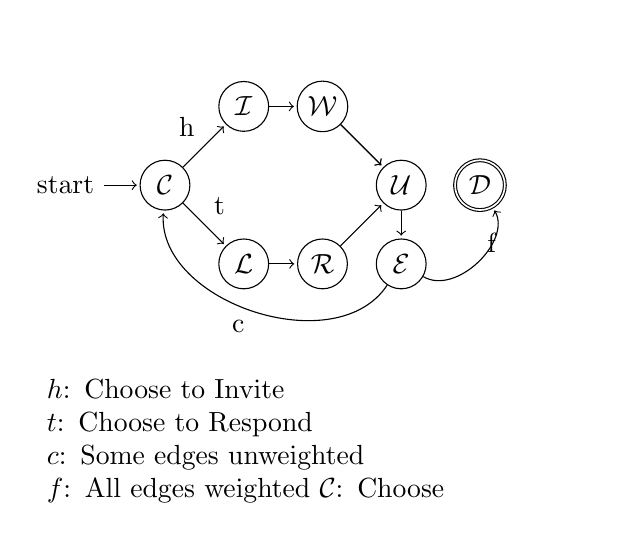
\begin{tikzpicture}[shorten >=1pt,node distance=1cm,on grid,auto, bend angle=75, every state/.style={scale=1, minimum size=18pt, inner sep=2pt}]
    %\draw [help lines] (0,-2) grid (4,2);
    \path [help lines] (0,-2) grid (4,2); 
    \node [state, initial]   (C)          {\cCd};
    \node [state] (I)            at (1,1) {\cId};
    \node [state] (L)            at (1,-1) {\cLd};
    \node [state] (W)            at (2,1)       {\cWd};
    \node [state] (R)            at (2,-1)       {\cRd};
    \node [state] (U)            at (3,0) {\cUd};
    \node [state] (E)            at (3,-1)       {\cEd};
    \node [state, accepting] (D) at (4,0)   {\cDd};

    \path [->] (C) edge              node {h} (I)
                   edge              node {t} (L)
               (L) edge              node {} (R)
               (I) edge              node {} (W)
               (W) edge              node {} (U)
               (R) edge              node {} (U)
               (U) edge              node {} (E);
    \path [->] (E) edge [bend right] node [above right] {f} (D);
    \path [->] (W) edge              node {} (U);
    \path [->] (E) edge [bend left]  node {c} (C);


      \node [text width=7cm] (key) at (2, -3.25) {
	$h$: Choose to Invite \hspace{4cm}
        $t$: Choose to Respond\hspace{4cm}
        $c$: Some edges unweighted\hspace{5cm}
	$f$: All edges weighted
	$\cC$: Choose 
	}; 
  \end{tikzpicture}
  \end{center}
  \label{fig:dgmm-auto}
\end{figure}


Each vertex begins in the \cCd\ state, and chooses to either send invitations (\cId), or listen for invitation (\cLd). Vertices in the \cId\ state choose one neighbor to send an invitation to and transition to a waiting state (\cWd), and vertices in the \cLd\ state choose one invitation to accept. The acceptence message is sent during the response state \cRd. All vertices then update their status (\cUd). Vertices that have either chosen to join the cover or which have no undecided neighbors will transition to the done state, (\cDd), and other vertices return to state \cCd.  


During the \cUd\ state, vertex pairs formed during the invitation/acceptance phases are able to assign a weight to the edge between them independently using equation~\ref{eqn:gmm}, and therefore decide whether or not to join the cover. During the \cEd\ state neighboring vertices are able to update some of their own edge weights, by assigning a weight of zero to any edges incident to a vertex which has joined the cover.

\begin{algorithm}
\caption{Distributed Weighted Vertex Cover}
\begin{algorithmic}
\Require {$G(V,E)$: a graph}
\ForAll {$v_u \in V$ in parrallel}
\State $S_u \leftarrow False$
\State state $\leftarrow$ Choose
\Repeat
\State Broadcast $S_u$
\If {$S_v = True$ for $v_v$ incident to self}
\State Set Weight $e_{u,v} \leftarrow 0$
\EndIf
\If {state = Choose}
\State {Choose A State (Invite, Listen)}
\ElsIf {state = Invite}
\State {Select an unweighted edge, $e_{u,v}$}
\State {Broadcast an Invitation to $v_v$}
\State {state $\leftarrow$ Wait}
\ElsIf {state = Listen}
\State {Collect Invitations}
\State {state $\leftarrow$ Respond}
\ElsIf {state = Wait}
\State {Collect Responses}
\If {Response Matches Invitation}
\State {Update Weight $e_{u,v}$}
\If {$\sum_{w_e} e incident v_u = w_u$}
\State $S_u \leftarrow true$
\EndIf
\EndIf
\State {state $\leftarrow$ Choose}
\ElsIf {state = Respond}
\State Choose Invitation, Broadcast Response
\State {Update Weight $e_{u,v}$}
\If {$\sum_{w_e} e incident v_u = w_u$}
\State $S_u \leftarrow true$
\EndIf
\State {state $\leftarrow$ Choose}
\EndIf
\Until {$S_u = true$ OR $S_v = true$ for all $v_v$ incident $v_u$}
\EndFor
\end{algorithmic}
\label{alg:dgmm}
\end{algorithm}

\subsection{Performance}
\begin{thm}
  Algorithm~\ref{alg:dgmm} (DGMM) will generate a 2-optimal cover in $O(log \Delta)$ communication rounds with high probability on any input.
\label{thm:dgmm-term}
\end{thm}
\begin{smy}
We show first that our algorithm conducts the same steps in the same order as a sequential algorithm that is known to produce a 2-optimal result, next that the algorithm will terminate in $O(log \Delta)$ communication rounds.
\end{smy} 

\begin{note}[Communication Model]
\label{not:com-model}
As mentioned in Section~\ref{ssb:com-model}, we assume a message passing model of distributed computing. In each communication round, it is assumed that every node can communicate with its neighbors. Communication is assumed to be synchronous and symetric: if node $a$ is a neighbor of node $b$, node $b$ is a neighbor of node $a$, and if node $a$ has counted $x$ communication steps, so has node $b$.

A ``communication round'' is actually three steps: an invitation sending step, an information response step, and an exchange step where neighbors share changes in status.\footnote{It should be noted that the K/Y algorithm also requires three communication events per round.} 
\end{note}
\begin{note}[Local Information]
\label{not:dgmm-local-info}
At the beginning of each communication round, each node has a list of its neighbors, their current state, the edges associated with those neighbors, and the results of any previous computation performed on those edges.
\end{note}
\begin{note}[Mapping to Sequential Algorithm]
\label{not:gmm-dgmm}
DGMM is based on a sequential algorithm (GMM), which takes as an input a graph and produces a 2-optimal vertex cover of that graph. The sequential algorithm selects each edge of the graph in turn, in arbitrary order, and compares the endpoints of that edge. The edge is assigned a weight according to Equation~\ref{eqn:gmm}. If one endpoint is already in the cover, the resulting weight will be zero, otherwise, one endpoint will be added to the cover. When each edge has been assigned a weight, the algorithm terminates and outputs the cover.

For DGMM, the Graph is represented as a network of compute nodes, with the nodes representing vertices and connections between the nodes representing edges. Nodes form pairs over these connections and assign weights to each connection following the same rules as the sequential algorithm. A node that joins the cover turns itself "on", while nodes turn off if they have no unweighted edges and have not joined the cover. When the algorithm terminates, every node in the network that is in the cover will be in an ``on'' state, and every node that is not will be in an ``off'' state.
\end{note}

\begin{proof}[Proof of Theorem~\ref{thm:dgmm-term}]
\label{prf:correct}

\begin{lem}
\label{lem:dgmm-edge}
  DGMM weights each edge once in a manner equivalent to GMM.
\end{lem}
\begin{proof}[Proof of Lemma~\ref{lem:dgmm-edge}]
  Lemma~\ref{lem:dgmm-edge} can be restated in terms of the following propositions.
  \begin{lprp}
    \label{prop:dgmm-edge-order}
    Given a matching, a simultaneous weighting of the edges in that matching is equivalent to an arbitrary sequential weighting of the same edges.
  \end{lprp}
  \begin{lprp}
    \label{prop:dgmm-edge-match}
    DGMM produces a matching in each communication round.
  \end{lprp}
  \begin{lprp}
    \label{prop:dgmm-edge-once}
    DGMM weights every edge exactly once.
  \end{lprp}
  If these propositions are true, Lemma~\ref{lem:dgmm-edge} is also true. 
  
  \begin{proof}[Proof of Proposition~\ref{prop:dgmm-edge-order}]
    By definition of a matching, no two edges in a matching share a vertex. Therefore, if an edge $e(u,v)$ is in the matching, no edge $e(u,i)$ is in the matching. 
    Take a matching \bMd\ in a Graph $G(V,E)$, composed of edges $\{e_0, e_1, ..., e_n\}$. If we use the sequential algorithm to weight the edges in \bMd\ one after the other according to~\eqref{eqn:gmm} (page~\pageref{eqn:gmm}), it is obvious that no edge outside of \bMd\ will change. Since only edges outside of \bMd\ are used to assign weights to edges inside \bMd\, it does not matter what order the weights are assigned in, or whether the weight assignment occurs to all edges in \bMd\ simultaneously.
    
    Therefore Proposition~\ref{prop:dgmm-edge-order} is true.
  \end{proof}
  \begin{proof}[Proof of Proposition~\ref{prop:dgmm-edge-match}]
    Assume not, that is, assume that there are two edges $e(u,v) \text{ and } e(u,i)$ that are both updated during the same communication round. For this to happen, some compute node $u$ must form a partnership with two nodes $i$ and $v$. 
    
At the beginning of every communication round, each node makes an equally weighted random decision to either issue an invitation or wait for invitations. We consider these options by cases.

    Case One: Assume that $v$ issues invitations. If $v$ issues invitations, $v$ will choose a single unweighted edge $(v,u)$ and broadcast an invitation with the id of $u$ to all of its neighbors (Line~\algref{alg:dgmm}{alglin:dgmm-issue-invite}). $v$ then transitions to the \cWd\ state. In this state, the node gathers all responses issued by its neighbors, and updates an edge if a response is sent specifically to .

    So if two edges are weighted, $v$ must receive two responses.

    Responses are issued by nodes in the \cRd\ state. Each node in this state chooses a single invitation from its received invitations and responds to it. Since $v$ gets two responses, therefore, $v$ must have invited two separate nodes in this round. But $v$ only issues one invitation, so this is a contradiction.

    Case Two: Assume that $v$ receives invitations. A node which recieves invitations updates the edge corresponding to the invitation it recieved. Since $v$ is weighting two edges, $v$ must respond to multiple invitations in this round. However, $v$ only sends a single response message (Line~\algref{alg:dgmm}{alglin:dgmm-choose-invite}), which is a contradiction as well.
    Therefore, Proposition~\ref{prop:dgmm-edge-match} is true.
  \end{proof}
  \begin{proof}[Proof of Proposition~\ref{prop:dgmm-edge-once}]
    Because a node will only attempt to weight an unweighted edge, we know that no edge will be weighted more than once. If the proposition is false, it must be the case that some edge is not weighted.
    For an edge to be unweighted, both endpoints of the edge would have to halt (enter the \cDd\ state) before the edge is weighted. Nodes halt under two circumstances:
    \begin{enumerate}
    \item The node has joined the cover.
    \item A node's neighbors have all joined the cover.
    \end{enumerate}
    In the first case, the node will weight all of its unweighted edges to 0. In the second case, the node weights its own edges to 0 if the other endpoint is in the cover.
    Therefore, if the algorithm halts, all edges have been weighted once.
  \end{proof}
  Therefore, Lemma~\ref{lem:dgmm-edge}: our algorithm weights edges equivalently to the GMM algorithm. As we have indicated, prior work by Gonzalez has shown GMM to be 2-optimal, therefore we have the following corallary.
\begin{cor}\label{cor:dgmm-two}DGMM is two optimal.\end{cor}
\end{proof}


\begin{lem}
  \label{lem:dgmm-delta}
  DGMM will weight all edges in approximately $log\Delta$ communication rounds with high probability.
\end{lem}

\begin{ldef}
A node is {\em committed} if it has joined the cover or if all of its neighbors have joined the cover.
\end{ldef}
\begin{ldef}
A node is {\em active} if it is not committed.
\end{ldef}
\begin{ldef}
$\Delta$ is the maximum degree of the Graph.
\end{ldef}
\begin{ldef}
\label{def:gamma}
For an active node $u$, $\Gamma_u$ is the number of uncovered edges of $u$. $\Gamma$ is the average value of $\Gamma_u$ for all active nodes in the Graph. $\Gamma_u$ is equivalent to the number of active neighbors of $u$, and is bounded by $\Delta$.
\end{ldef}
\begin{note}
Only nodes that are still active at the end of a round participate in the next round. 
\end{note}
 
\begin{IEEEproof}[Proof of Lemma~\ref{lem:dgmm-delta}]
The neighborhood of $u$ ($N_u$) contains $u$ and all nodes $v$ such that there is an edge $(u,v)$. We can assume without loss of generality that there are $\Gamma$ uncovered edges and therefore $\Gamma$ active nodes in $N_u$. $u$ must cover all of these edges in order for the algorithm to halt. 

If $u$ joins the cover in a round, all of its edges will be covered. Otherwise, an edge $(u,v)$ will be covered only if $v$ joins the cover.

At the beginning of a round, $u$ chooses to issue invitations or recieve invitations without bias.

Assume $u$ chooses to recieve invitations. Approximately $\sfrac{\Gamma}{2}$ of the active neighbors of $u$ will choose to send invitations. We can assume that for each node $v$ that is a neighbor of $u$, $\Gamma_v = \Gamma$. Each sender chooses one of its $\Gamma$ active nodes to send an invitation to without bias, so the odds that a given neighbor of $u$ will send an invitation to $u$ is $\sfrac{\Gamma}{2} \times \sfrac{1}{\Gamma} = \sfrac{1}{2}$. If $u$ recieves any invitations, it will respond to at least one. We know that if $u,v$ are endpoints in the matching for a round, one of them must join the cover, so if $u$ is a reciever, it will cover at least one edge with a probability of $\sfrac{1}{2}$. The probability that $u$ will join the cover is the same as the probability that $v$ will join the cover, so $u$ will cover all of its edges with a probability of $\sfrac{1}{2}$. Therefore, the probability that $u$ is a reciever and all edges incident to $u$ are covered is $\sfrac{1}{2} \times \sfrac{1}{2} \times \sfrac{1}{2} = \sfrac{1}{8}$.

For each active neighbor of $u$, this same analysis applies. Each node will be a reciever with probability of $\sfrac{1}{2}$ and each node that is a reciever will weight all of its edges with a probability of $\sfrac{1}{4}$.

Assume that $u$ is dormant for all phases of the round except the exchange/update phase. In this phase, all nodes that have joined the cover broadcast their status. If $u$ is incident to a node $v$ that joins the cover and edge $(u,v)$ is unweighted, $u$ will set the weight of $(u,v)$ to 0. 

$\sfrac{\Gamma_u}{2}$ neighbors of $u$ will choose to be recievers. Of these, $\sfrac{1}{2}$ will participate in the matching. Of these, $\sfrac{1}{2}$ will join the cover.

Therefore, during the exchange phase, every node $u$ will weight $\sfrac{\Gamma_u}{2} \times \sfrac{1}{2} \times \sfrac{1}{2} = \sfrac{\Gamma}{8}$ of its edges in every round regardless of whether $u$ joins the matching or not. 

$\Gamma$ is bounded by $\Delta$, and the algorithm terminates when all nodes have weighted all edges. Therefore Lemma~\ref{lem:dgmm-delta} is correct.
\end{IEEEproof}


Therefore, because DGMM weights all edges and assigns nodes to the cover in a manner equivalent to GMM in $O(log \Delta)$ communication rounds, Theorem~\ref{thm:dgmm-term} is proved.
\end{proof}

\bibliography{vertex_bib}
\end{document}

